% DEFINITION
Due to the lack of a universally accepted terminology, we define a \textit{multilevel} or \textit{hierarchical model} as ``an assembly of submodels at different levels of a hierarchy''.
The hierarchical structure can be constituted by stochastic dependencies and deterministic maps between the quantities involved.
% GENERAL
According to that definition multilevel modeling forms sort of an overarching theme in modern cross-disciplinary statistics.
In the last two decades it has been extensively studied from a frequentist \cite{Multilevel:Davidian2003,Multilevel:Banks2012} and a Bayesian \cite{Multilevel:Wakefield1996,Multilevel:Lunn2005} point of view.
% ISSUES
Adopting the latter paradigm, prior elicitation \cite{Multilevel:Daniels1999,Multilevel:Gelman2006:b}
and posterior computation \cite{MCMC:Wakefield1994,MCMC:Bennett1995} are delicate issues that have been discussed in the statistical literature.
% APPLICATIONS
Applications of multilevel modeling encompass probabilistic inversion \cite{Nagel:IPW2013:Proc,Multilevel:Ballesteros2014:Proc} and optimal combination of information \cite{Multilevel:Draper1992,Nagel:ICVRAM2014:Proc}.
% UNCERTAINTY
Based on a probabilistic representation of both epistemic uncertainty and aleatory variability,
% INVERSION
Bayesian multilevel modeling establishes a natural framework for solving complex inverse problems under uncertainty.
% INFERENCE
Inference can be accomplished by transforming, conditioning and marginalizing probability distributions.

\subsection{Uncertainty and variability} \label{sec:JAIS:Multilevel:Uncertainty}
% FORWARD MODEL
A \textit{forward model} \(\mathcal{M} \colon (\bm{m},\bm{x},\bm{\zeta},\bm{d}) \mapsto \perfect{\bm{y}}\) represents the system or phenomenon under consideration.
It formally maps model inputs \((\bm{m},\bm{x},\bm{\zeta},\bm{d}) \in \mathcal{D}_{\bm{m}} \times \mathcal{D}_{\bm{x}} \times \mathcal{D}_{\bm{\zeta}} \times \mathcal{D}_{\bm{d}}\)
to outputs \(\perfect{\bm{y}}=\mathcal{M}(\bm{m},\bm{x},\bm{\zeta},\bm{d}) \in \mathcal{D}_{\perfect{\bm{y}}} \subset \mathds{R}^d\).
% EXPERIMENTS
When carrying out a number of experiments the variability of measured forward model responses can be attributed to models of input uncertainty.
There are fixed yet unknown model parameters \(\bm{m} \in \mathcal{D}_{\bm{m}} \subset \mathds{R}^p\),
model inputs \(\bm{\zeta} \in \mathcal{D}_{\bm{\zeta}} \subset \mathds{R}^r\) with perfectly known aleatory variability,
input variables \(\bm{x} \in \mathcal{D}_{\bm{x}} \subset \mathds{R}^q\) with imperfectly known aleatory variability,
and experimental conditions \(\bm{d} \in \mathcal{D}_{\bm{d}} \subset \mathds{R}^s\) that are entirely known.
\par % PROBABILISTIC REPRESENTATION
With respect to a number of \(i=1,\ldots,n\) experiments, forward model inputs are represented as deterministic or stochastic objects within the Bayesian multilevel framework.
% EXPERIMENTAL CONDITIONS
Throughout the experiments data is acquired under known but possibly different experimental conditions \(\bm{d}_i\).
These model inputs \(\bm{d}_i\) are therefore deterministically represented.
% FIXED ALBEIT UNKNOWN
Fixed albeit unknown model parameters \(\bm{m}\) are assumed to be constant over the experiments.
In Bayesian fashion they are represented as random variables \(\bm{M} \sim \pi_{\bm{M}} (\bm{m})\),
where the Bayesian prior distribution \(\pi_{\bm{M}} (\bm{m})\) accounts for a subjective degree of belief or prior knowledge about their true values.
This is the Bayesian conception of \textit{epistemic uncertainty}.
\par % PRECISE DISTRIBUTION
Over the number of experiments varying model inputs \(\bm{\zeta}\) take on unknown experiment-specific realizations \(\bm{\zeta}_i\) of conditionally independent
random variables \((\bm{Z}_i \cond \bm{\theta}_{\bm{Z}}) \sim f_{\bm{Z} \cond \bm{\Theta}_{\bm{Z}}}(\bm{\zeta}_i \cond \bm{\theta}_{\bm{Z}})\).
The conditional distribution \(f_{\bm{Z} \cond \bm{\Theta}_{\bm{Z}}}(\bm{\zeta}_i \cond \bm{\theta}_{\bm{Z}})\) with known hyperparameters \(\bm{\theta}_{\bm{Z}}\)
states a subjective degree of belief or prior knowledge about the individual realizations \(\bm{\zeta}_i\).
This is a Bayesian notion of \textit{aleatory variability}.
% IMPRECISE DISTRIBUTION
Similarly model inputs \(\bm{x}\) are subject to variability and take on unknown experiment-specific realizations \(\bm{x}_i\)
of conditionally independent random variables \((\bm{X}_i \cond \bm{\theta}_{\bm{X}}) \sim f_{\bm{X} \cond \bm{\Theta}_{\bm{X}}} (\bm{x}_i \cond \bm{\theta}_{\bm{X}})\).
The hyperparameters \(\bm{\theta}_{\bm{X}}\) determine this variability throughout the experiments and are fixed but unknown.
In turn they are modeled as random variables \(\bm{\Theta}_{\bm{X}} \sim \pi_{\bm{\Theta}_{\bm{X}}} (\bm{\theta}_{\bm{X}})\),
where the distribution \(\pi_{\bm{\Theta}_{\bm{X}}} (\bm{\theta}_{\bm{X}})\) quantifies an a priori degree of plausibility.
% EXCHANGEABILITY
Random variables \((\bm{X}_1,\ldots,\bm{X}_n) \sim \int (\prod_{i=1}^n f_{\bm{X} \cond \bm{\Theta}_{\bm{X}}} (\bm{x}_i \cond \bm{\theta}_{\bm{X}})) \,
\pi_{\bm{\Theta}_{\bm{X}}} (\bm{\theta}_{\bm{X}}) \, \mathrm{d} \bm{\theta}_{\bm{X}}\) embody the prior knowledge about the experiment-specific realizations \(\bm{x}_i\).
\par % INTERPRETATION: PARAMETRIC & STRUCTURAL PRIOR KNOWLEDGE
Summarizing, marginal distributions \(\pi_{\bm{M}} (\bm{m})\) and \(\pi_{\bm{\Theta}_{\bm{X}}} (\bm{\theta}_{\bm{X}})\)
represent \textit{parametric prior knowledge} about the true values of the model parameters \(\bm{m}\) and the hyperparameters \(\bm{\theta}_{\bm{X}}\),
whereas conditional distributions \(f_{\bm{X} \cond \bm{\Theta}_{\bm{X}}}(\bm{x}_i \cond \bm{\theta}_{\bm{X}})\) and \(f_{\bm{Z} \cond \bm{\Theta}_{\bm{Z}}}(\bm{\zeta}_i \cond \bm{\theta}_{\bm{Z}})\)
encapsulate \textit{structural prior knowledge} about the problem, i.e.\ information about experiment-specific \(\bm{x}_i\) and \(\bm{\zeta}_i\).

\subsection{Statistical data model} \label{sec:JAIS:Multilevel:Overall}
% MODEL IMPERFECTION
An integral constituent of many statistical approaches to inverse problems is a residual model.
Real observations \(\bm{y}_i\) often deviate from model predictions \(\perfect{\bm{y}}_i = \mathcal{M}(\bm{m},\bm{x}_i,\bm{\zeta}_i,\bm{d}_i)\) even if forward model inputs were known with certainty.
This discrepancy, which is due to measurement errors, numerical approximations and model inadequacies, is often accounted for by a statistical data model \(\bm{y}_i = \perfect{\bm{y}}_i + \bm{\varepsilon}_i\).
Prediction errors \(\bm{\varepsilon}_i\) are assumed to be realizations of random variables \(\bm{E}_i \sim f_{\bm{E}_i}(\bm{\varepsilon}_i)\), e.g.\ with normal distributions
\(f_{\bm{E}_i}(\bm{\varepsilon}_i) = \mathcal{N}(\bm{\varepsilon}_i \cond \bm{0},\bm{\Sigma}_i)\) and experiment-specific, symmetric and positive-semidefinite covariance matrices \(\bm{\Sigma}_i\).
It quantifies a degree of imperfection of the forward model and experimental apparatus.
% RANDOM DATA
Hence observations are viewed as realizations \(\bm{y}_i\) of random variables \((\bm{Y}_i \cond \bm{m},\bm{x}_i,\bm{\zeta}_i)\)
with distributions \(f (\bm{y}_i \cond \bm{m},\bm{x}_i,\bm{\zeta}_i) = f_{\bm{E}_i}(\bm{y}_i-\mathcal{M}(\bm{m},\bm{x}_i,\bm{\zeta}_i,\bm{d}_i))\).
% PROBABILISTIC MODEL
The overall model formulated thus far can be summarized as
\begin{subequations} \label{eq:JAIS:Multilevel:Model}
  \begin{align}
    (\bm{Y}_i \cond \bm{m},\bm{x}_i,\bm{\zeta}_i) &\sim f_{\bm{E}_i} \big( \bm{y}_i-\mathcal{M}(\bm{m},\bm{x}_i,\bm{\zeta}_i,\bm{d}_i) \big), \label{eq:JAIS:Multilevel:Model:Data} \\
    \bm{M} &\sim \pi_{\bm{M}} (\bm{m}), \label{eq:JAIS:Multilevel:Model:PriorM} \\
    (\bm{X}_i \cond \bm{\theta}_{\bm{X}}) &\sim f_{\bm{X} \cond \bm{\Theta}_{\bm{X}}} (\bm{x}_i \cond \bm{\theta}_{\bm{X}}), \label{eq:JAIS:Multilevel:Model:PopulationX} \\
    \bm{\Theta}_{\bm{X}} &\sim \pi_{\bm{\Theta}_{\bm{X}}} (\bm{\theta}_{\bm{X}}), \label{eq:JAIS:Multilevel:Model:PriorThetaX} \\
    (\bm{Z}_i \cond \bm{\theta}_{\bm{Z}}) &\sim f_{\bm{Z} \cond \bm{\Theta}_{\bm{Z}}}(\bm{\zeta}_i \cond \bm{\theta}_{\bm{Z}}). \label{eq:JAIS:Multilevel:Model:PopulationZ}
  \end{align}
\end{subequations}
\par % OVERALL JOINT DENSITY
This model is composed of conditional probabilistic and deterministic relations between the quantities involved.
As per our previous definition it is a generic Bayesian multilevel model.
% DAG
An intuitive model representation is provided by a directed acyclic graph (DAG) \cite{Bayesian:Koski2009,Bayesian:Kjaerulff2013}, such as shown in \cref{fig:JAIS:Multilevel:DAG}.
% OUTLOOK ON PERFECT DATA
In \cref{sec:JAIS:PerfectData} we will devise a model for analyzing ``perfect'' observations \(\perfect{\bm{y}}_i\) instead of the ``imperfect'' ones \(\bm{y}_i = \perfect{\bm{y}}_i + \bm{\varepsilon}_i\).
Unlike the latter, the randomness of the former is exclusively attributed to forward model input variability as discussed in \cref{sec:JAIS:Multilevel:Uncertainty}.
% INDEPENDENCE
Unless stated or denoted otherwise random variables in \cref{eq:JAIS:Multilevel:Model} are assumed to be (conditionally) independent.
This defines a joint overall probability density of all probabilistic quantities.
% CONDITIONING & MARGINALIZING
By conditioning and marginalizing this overall density at one's convenience, one can derive meaningful probability densities.
For inferential purposes these are certain prior and posterior distributions that we will explain in the following.
% DAG
\begin{figure}[htbp]
  \centering
  \includegraphics[height=\JAISdagHeight]{fig_JAIS_DAG_GENERIC}
  \caption[DAG of the generic multilevel model]{DAG of the generic multilevel model.
           Vertices symbolize unknown (\(\vcenter{\hbox{\protect\includegraphics[height=1.3ex]{fig_Circle}}}\))
           or known (\(\vcenter{\hbox{\protect\includegraphics[height=1.2ex]{fig_Square}}}\)) quantities
           and directed edges represent their deterministic (\(\vcenter{\hbox{\protect\includegraphics[height=1.0ex]{fig_Solid}}}\))
           or probabilistic (\(\vcenter{\hbox{\protect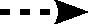
\includegraphics[height=1.0ex]{fig_Dashed}}}\)) relations.
           Model parameters \(\bm{m}\) are constant over \(i=1,\ldots,n\) experiments.
           The variability of experiment-specific realizations \(\bm{x}_i\) and \(\bm{\zeta}_i\) is determined
           by unknown or known hyperparameters \(\bm{\theta}_{\bm{X}}\) and \(\bm{\theta}_{\bm{Z}}\), respectively.
           Data can be interpreted as ``perfect'' \(\perfect{\bm{y}}_i = \mathcal{M}(\bm{m},\bm{x}_i,\bm{\zeta}_i,\bm{d}_i)\)
           or ``imperfect'' observations \(\bm{y}_i = \perfect{\bm{y}}_i + \bm{\varepsilon}_i\) with
           \(f_{\bm{E}_i}(\bm{\varepsilon}_i) = \mathcal{N}(\bm{\varepsilon}_i \cond \bm{0},\bm{\Sigma}_i)\).
          }
  \label{fig:JAIS:Multilevel:DAG}
\end{figure}

\subsection{Inference in multilevel models} \label{sec:JAIS:Multilevel:Inference}
% NOTATION
In what follows \(\tuple{\bm{q}_i}\) denotes a tuple \(\tuple{\bm{q}_i}_{1 \leq i \leq n} = (\bm{q}_1,\bm{q}_2,\ldots,\bm{q}_n)\).
% PRIOR
Conditioned on the priorly known hyperparameters \(\bm{\theta}_{\bm{Z}}\), the joint prior distribution of the unknowns \((\bm{m},\tuple{\bm{x}_i},\tuple{\bm{\zeta}_i},\bm{\theta}_{\bm{X}})\) is given as
\begin{equation} \label{eq:JAIS:Multilevel:Prior}
  \pi \big( \bm{m},\tuple{\bm{x}_i},\tuple{\bm{\zeta}_i},\bm{\theta}_{\bm{X}} \cond \bm{\theta}_{\bm{Z}} \big)
  = \left( \prod\limits_{i=1}^n f_{\bm{X} \cond \bm{\Theta}_{\bm{X}}}(\bm{x}_i \cond \bm{\theta}_{\bm{X}}) \right)
  \left( \prod\limits_{i=1}^n f_{\bm{Z} \cond \bm{\Theta}_{\bm{Z}}}(\bm{\zeta}_i \cond \bm{\theta}_{\bm{Z}}) \right)
  \pi_{\bm{\Theta}_{\bm{X}}} (\bm{\theta}_{\bm{X}})\, \pi_{\bm{M}} (\bm{m}).
\end{equation}
It summarizes the available parametric and structural prior knowledge.
% POSTERIOR
The joint posterior distribution of the unknowns \((\bm{m},\tuple{\bm{x}_i},\tuple{\bm{\zeta}_i},\bm{\theta}_{\bm{X}})\)
is obtained by further conditioning the prior \cref{eq:JAIS:Multilevel:Prior} on the data \(\tuple{\bm{y}_i}\).
By virtue of Bayes' law this posterior is up to a scale factor found as
\begin{equation} \label{eq:JAIS:Multilevel:Posterior}
  \pi \big( \bm{m},\tuple{\bm{x}_i},\tuple{\bm{\zeta}_i},\bm{\theta}_{\bm{X}} \cond \tuple{\bm{y}_i},\bm{\theta}_{\bm{Z}} \big)
  \propto \left( \prod\limits_{i=1}^n f_{\bm{E}_i} \big( \bm{y}_i-\mathcal{M}(\bm{m},\bm{x}_i,\bm{\zeta}_i,\bm{d}_i) \big) \right)
  \pi \big( \bm{m},\tuple{\bm{x}_i},\tuple{\bm{\zeta}_i},\bm{\theta}_{\bm{X}} \cond \bm{\theta}_{\bm{Z}} \big).
\end{equation}
% MARGINAL POSTERIOR
The posterior degree of plausibility about the \textit{quantities of interest} (QoI) can be extracted
by marginalizing the posterior \cref{eq:JAIS:Multilevel:Posterior} over parameters considered \textit{nuisance} \cite{Statistics:Basu1977:a,Statistics:Dawid1980:a}.
Provided \((\bm{m},\bm{\theta}_{\bm{X}})\) are QoI and \((\tuple{\bm{x}_i},\tuple{\bm{\zeta}_i})\) are nuisance parameters, the correspondingly marginalized posterior is
\begin{equation} \label{eq:JAIS:Multilevel:MarginalPosterior}
  \pi \big( \bm{m},\bm{\theta}_{\bm{X}} \cond \tuple{\bm{y}_i},\bm{\theta}_{\bm{Z}} \big) = 
  \int\limits_{\mathcal{D}_{\bm{x}}^n} \int\limits_{\mathcal{D}_{\bm{\zeta}}^n}
  \pi \big( \bm{m},\tuple{\bm{x}_i},\tuple{\bm{\zeta}_i},\bm{\theta}_{\bm{X}} \cond \tuple{\bm{y}_i},\bm{\theta}_{\bm{Z}} \big)
  \, \mathrm{d} \tuple{\bm{x}_i} \, \mathrm{d} \tuple{\bm{\zeta}_i},
\end{equation}
where \(\mathrm{d} \tuple{\bm{x}_i} = \mathrm{d} \bm{x}_1 \ldots \mathrm{d} \bm{x}_n\) and \(\mathrm{d} \tuple{\bm{\zeta}_i} = \mathrm{d} \bm{\zeta}_1 \ldots \mathrm{d} \bm{\zeta}_n\).
% SUMMARY
Summarized the genuinely unique approach to Bayesian inference in multilevel models is to construct the posterior of the QoI \((\bm{m},\bm{\theta}_{\bm{X}})\)
by conditioning on the knowns \((\tuple{\bm{y}_i},\bm{\theta}_{\bm{Z}})\) and subsequently marginalizing out nuisance \((\tuple{\bm{x}_i},\tuple{\bm{\zeta}_i})\).

\subsection{Marginalized formulation}
% \par % MARGINALIZED FORMULATION
Equivalently one could solve a marginal formulation of the multilevel calibration problem,
with a marginal prior \(\pi(\bm{m},\bm{\theta}_{\bm{X}}) = \pi_{\bm{M}} (\bm{m}) \, \pi_{\bm{\Theta}_{\bm{X}}} (\bm{\theta}_{\bm{X}})\)
and a marginalized version of the likelihood \(\mathcal{L}(\tuple{\bm{y}_i} \cond \bm{m},\bm{\theta}_{\bm{X}}, \bm{\theta}_{\bm{Z}})\) \cite{Statistics:Berger1999,Statistics:Severini2007}.
% MARGINALIZED FORMULATION
One therefore factorizes the marginalized posterior \cref{eq:JAIS:Multilevel:MarginalPosterior} as
\begin{equation} \label{eq:JAIS:Multilevel:Marginal:Factorization}
  \pi \big( \bm{m},\bm{\theta}_{\bm{X}} \cond \tuple{\bm{y}_i},\bm{\theta}_{\bm{Z}} \big)
  \propto \left( \prod_{i=1}^n f(\bm{y}_i \cond \bm{m},\bm{\theta}_{\bm{X}},\bm{\theta}_{\bm{Z}}) \right) \pi_{\bm{M}} (\bm{m}) \, \pi_{\bm{\Theta}_{\bm{X}}} (\bm{\theta}_{\bm{X}}),
\end{equation}
where \(f(\bm{y}_i \cond \bm{m},\bm{\theta}_{\bm{X}},\bm{\theta}_{\bm{Z}})\) is the marginalized density of the observation \(\bm{y}_i\).
The aleatory variables \((\bm{x}_i,\bm{\zeta}_i)\) have been eliminated based on the integration
\begin{equation} \label{eq:JAIS:Multilevel:Marginal:Marginalization}
  f(\bm{y}_i \cond \bm{m},\bm{\theta}_{\bm{X}},\bm{\theta}_{\bm{Z}}) = \int\limits_{\mathcal{D}_{\bm{x}}} \int\limits_{\mathcal{D}_{\bm{\zeta}}}
  f_{\bm{E}_i} \big( \bm{y}_i-\mathcal{M}(\bm{m},\bm{x}_i,\bm{\zeta}_i,\bm{d}_i) \big) \, f_{\bm{X} \cond \bm{\Theta}_{\bm{X}}} (\bm{x}_i \cond \bm{\theta}_{\bm{X}})
  \, f_{\bm{Z} \cond \bm{\Theta}_{\bm{Z}}}(\bm{\zeta}_i \cond \bm{\theta}_{\bm{Z}}) \, \mathrm{d} \bm{x}_i \, \mathrm{d} \bm{\zeta}_i.
\end{equation} 
When defining the \textit{marginalized} or \textit{integrated likelihood} as 
\(\mathcal{L}(\tuple{\bm{y}_i} \cond \bm{m},\bm{\theta}_{\bm{X}}, \bm{\theta}_{\bm{Z}}) = \prod_{i=1}^n f(\bm{y}_i \cond \bm{m},\bm{\theta}_{\bm{X}},\bm{\theta}_{\bm{Z}})\),
the marginal posterior \cref{eq:JAIS:Multilevel:Marginal:Factorization} simply writes as \(\pi(\bm{m},\bm{\theta}_{\bm{X}} \cond \tuple{\bm{y}_i},\bm{\theta}_{\bm{Z}}) \propto
\mathcal{L}(\tuple{\bm{y}_i} \cond \bm{m},\bm{\theta}_{\bm{X}}, \bm{\theta}_{\bm{Z}}) \, \pi(\bm{m},\bm{\theta}_{\bm{X}})\).
% NUMERICAL INTEGRATION
Directly computing the marginal posterior \cref{eq:JAIS:Multilevel:MarginalPosterior} involves a lower-dimensional parameter space compared to computing the joint posterior \cref{eq:JAIS:Multilevel:Posterior}.
However, it requires the computation of the integrals in \cref{eq:JAIS:Multilevel:Marginal:Marginalization}.